\section{Nix/NixOS}

To achieve our goal of making our system reproducible and buildable with a single command (See Implementation \ref{sect:buildsystem}) we have used the Nix package manager. It would not be an understatement to say this would have been impossible without Nix. Nix can be likened to the Python package manager 'pip,' but with significantly enhanced capabilities and applicability that extend beyond just package management to encompass the entire system environment.

\subsection{Introduction to Nix}

\textbf{Nix} \cite{dolstra2004nix} is an open-source, "purely functional package manager” used in Unix-like operating systems to provide a functional and reproducible approach to package management. Started in 2003 as a research project Nix \cite{dolstra2006purely} is widely used in both industry \cite{NixCommunityNixOSWiki} and academia \cite{10.1145/3152493.3152556} \cite{https://doi.org/10.1002/qua.26872} \cite{LHCbNix}, and its associated public package repository \texttt{nixpkgs} \cite{NixPkgs} as of Jan 2024 has over 80,000 unique packages making it the largest up-to-date package repository in the world  \cite{Marakasov_2024}. Out of Nix has also grown \textbf{NixOS} \cite{10.1145/1411204.1411255} a Linux distribution that is conceived and defined as a deterministic and reproducible entity that is declared functionally and is built using the \textbf{Nix} package manager. \\

Nix packages are defined in the \textbf{Nix Language} a lazy functional programming language where packages are treated like purely functional values that are built by side effect-less functions and once produced are immutable. Packages are built with every dependency down to the \texttt{ELF} interpreter and \texttt{libc} (C standard library) defined in nix. All packages are installed in the store directory, typically \texttt{/nix/store/} by their unique hash and package name as can be seen in Fig~\ref{fig:nix-store-path} as opposed to the traditional Unix Filesystem Hierarchy Standard (FHS).

%% Nix Store Path
\begin{figureBox}[label={fig:nix-store-path}, width=0.8\linewidth]{Nix Store Path}
  \begin{tabbing}
    \={\color{Purple}\texttt{/nix/store/}}\={\color{RoyalBlue}\texttt{sbldylj3clbkc0aqvjjzfa6slp4zdvlj}}-\={\color{Orange}\texttt{hello-2.12.1}} \\
    \>\small{Prefix} \>\small {Hash part} \>\small {Package name}
  \end{tabbing}
\end{figureBox}

Package source files, like tarballs and patches, are also downloaded and stored with their hash in the store directory where packages can find them when building. Changing a package's dependencies results in a different hash and therefore location in the store directory which means you can have multiple versions or variants of the same package installed simultaneously without issue. This design also avoids "DLL hell" by making it impossible to accidentally point at the wrong version of a package. Another important result is that upgrading or uninstalling a package cannot ever break other applications. \\

Nix builds packages in a sandbox to ensure they are built exactly the same way on every machine by restricting access to nonreproducible files, OS features (like time and date), and the network \cite{nixcon-sandboxs}. A package can and should be pinned to a specific NixOS release (regardless of whether you are using NixOS or just the package manager). This means that once a package is configured to build correctly it will continue to work the same way in the future, regardless of when and where it is used and it will never not be able to be built. \\

These features are extremely useful for scientific work, CERN uses Nix to package the LHCb Experiment because it allows the software "to be stable for long periods (longer than even long-term support operating systems)" and it means that as Nix is reproducible; all the experiments are completely reproducible as all bugs that existed in the original experiment stay and ensure the accuracy of the results \cite{LHCbNix}. \\

To create a package Nix evaluates a \textbf{derivation} which is a specification/recipe that defines how a package should be built. It includes all the necessary information and instructions for building a package from its source code, such as the source location, build dependencies, build commands, and post-installation steps. By default, Nix uses binary caching to build packages faster, the default cache is \texttt{cache.nixos.org} is open to everyone and is constantly being populated by CI systems. You can also specify custom caches. The basic iterative process for building Nix packages can be seen in Fig~\ref{fig:nix-derivation-loop}.

\begin{figureBox}[label = {fig:nix-derivation-loop}, width=0.8\linewidth]{Nix Build Loop}
  { \footnotesize
  \begin{enumerate} [itemsep=-0.2em]
    \item A hash is computed for the package derivation and, using that hash, a Nix store path is generated, e.g \nixstore[sbldylj3clbkc0aqvjjzfa6slp4zdvlj]{hello-2.12.1}.
    \item  Using the store path, Nix checks if the derivation has already been built. First, checking the configured Nix store e.g {\color{Purple}\texttt{/nix/store/}} to see if the path e.g {\color{RoyalBlue}\texttt{sbldylj3clbkc0aqvjjzfa6slp4zdvlj}}-{\color{Orange}\texttt{hello-2.12.1}} already exists. If it does, it uses that, if it does not it continues to the next step.
    \item Next it checks if the store path exists in a configured binary cache, this is by default \texttt{cache.nixos.org}. If it does it downloads it from the cache and uses that. If it does not it continues to the next step.
    \item Nix will build the derivation from scratch, recursively following all of the steps in this list, using already-realized packages whenever possible and building only what is necessary. Once the derivation is built, it is added to the Nix store.
  \end{enumerate}
  }
\end{figureBox}

\subsection{Example of a Nix package}

To give an example of what a Nix package might look like. We have created a flake (one method of defining a package) in Listing~\ref{list:nix-flake} that builds a version of the classic example package "hello". 

\codeBoxFile[label = {list:nix-flake}]{nix}{./background/code/hello.nix}{flake.nix}

To dive deeper into what each line does we have given a breakdown below for the \texttt{flake.nix}
{ \small
\begin{itemize}[itemsep=-0.25em]
  \item \textbf{Line 2:} We have specified that we want to build our flake with the stable \textbf{nix channel} \texttt{nixos-23.11}, the most recent channel at the time of writing. This "channel" is just a release branch on the \texttt{nixpkgs} GitHub repository. Channels do receive conservative updates such as bug fixes and security patches but no major updates after the initial release. The first time we build the hello package from our \texttt{flake.nix} a \texttt{flake.lock} is automatically generated that pins us to a specific revision of \texttt{nixos-23.11}. Our built inputs will not change until we relock our flake to either a different revision of \texttt{nixos-23.11} or a new channel entirely. 

  \item \textbf{Line 5:} Here we define \texttt{outputs} as a function that accepts, \texttt{self} (the flake) and \texttt{nixpkgs} (the set of packages we just pinned to on line 2). Nix will resolve all inputs, and then call the \texttt{output} function.
  
  \item \textbf{Line 6:} Here we specify that we are defining the default package for users on \texttt{x86\_64-linux}. If we tried to build this package on a different CPU architecture like for example ARM (\texttt{aarch64-linux}) the flake would refuse to build as the package has not been defined for ARM yet. If we desired we could fix this by adding a \texttt{defaultPackage.aarch64-linux} definition.

  \item \textbf{Line 7-9:} Here we are just defining a shorthand way to refer to x86 Linux packages. This syntax is similar if not identical to Haskell.

  \item \textbf{Line 10:} Here we begin the definition of the derivation which is the instruction set Nix uses to build the package.
  
  \item \textbf{Line 14:} We specify here that we need \texttt{gcc} in our sandbox to build our package. \texttt{gcc} here is shorthand for \texttt{gcc12} but we could specify any c compiler with any version of that compiler we liked. If you desired you could compile different parts of your package with different versions of GCC.

  \item \textbf{Line 15:} Here we are slightly abusing the configure phase to generate a hello.c file. You would usually download a source to build from with a command like \texttt{fetchurl} while providing a hash. Each phase is essentially run as a bash script. Everything inside \texttt{mkDerivation} is happening inside a sandbox that will be discarded once the package is built (technically after we garbage collect). 
  
  \item \textbf{Line 16:} Here we actually build our package
  
  \item \textbf{Line 17:} In this line we copy the executable we have generated which is currently in the sandbox into the actual package we are producing which will be in the store directory \texttt{/nix/store}. 
\end{itemize}
}
Below we have given some examples of how to run and investigate our hello package in Listing~\ref{list:nix-terminal}.

\codeBoxFile[label = {list:nix-terminal},  width=0.75\linewidth]{shell}{./background/code/hello-nix.sh}{Terminal}

In Fig~\ref{fig:dependency-graph} we can see the package dependency graph of our \texttt{hello} package. We are only dependent on 4 packages \texttt{libunistring}, \texttt{libidn2}, \texttt{xgcc}, \texttt{glibc} all of which Nix have installed and configured separately the rest of the non-nix system (assuming we are not on NixOS). 

\begin{figureBox}[label = {fig:dependency-graph}, width=0.6\linewidth]{Dependency graph}
  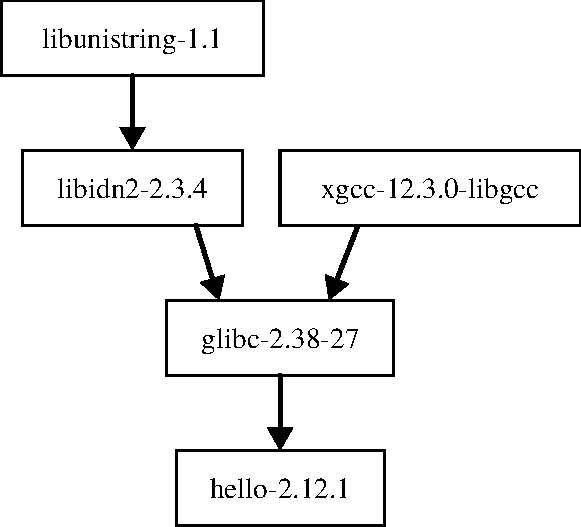
\includegraphics[width=0.7\linewidth]{./background/figures/nix/hello-pkg.pdf}
\end{figureBox}
